\documentclass{article}
\usepackage[utf8]{inputenc}
\usepackage{amsmath}
\usepackage{graphicx}
\graphicspath{  {./Figures/}  } 


% Outline
\iffalse
Title Page
Letter of Intent
Executive Summary
Table of Contents
List of Symbols
List of Figures
List of Tables
Introduction
	Background
	Objectives
Test Apparatus and Procedure
	Apparatus
	Procedure
Data Reduction Procedure
Results and Discussion
Conclusions and Recommendations
What I learned
References
Appendices

Executive summary
	- objectives: transform strain data to stress data
	- compare to theoretical analysis
	- data of significant/main findings: explain validity of data and meaning. 
	- limited by equipment, theoretical definition assumptions,

Background !!! site 3 articles!
	- basic background/ what about pressure vessels.
	- history of pressure vessels ?? Articles
	- linear relationship between pressure and stress.
	- how strain gages work: electrical resistance w/ deformation
	- Internal pressure leads to stresses experienced on walls

Objectives
	- gain hands on experience with materials and theory .
	- relationship between internal pressure and resultant strain
	- gather strain measurements with the rosettes
	- reduce the data to principal stresses and directions
	- compare rosette configurations, determine rosette validity and smart location. 
	- Analyze data: determine general validity.

Apparatus
	- Take pictures of equipment
	- strain rosette configuration
	- explain Rosette configurations and expected similiarities. 
	- give material properties: young's and poissons, strain rosette resistances?

Test Procedure
	- Zeroing the data and using normalized data
	- Starting at 0 psig and moving to 400, then reversing, using a hand pump.
	- Excel workbook, collecting mean shot of data.
	- Explain always what you expect.

Data Reduction: include equations here. 
	- show generalized process and data flow from rosette to stress.
	- list equations here
	- Rosette comparison values based on what is expected.
	- standard error, regression,
	- rosette C average, explain the expected values and why.
	- axial vs hoop: 2.0 per rosette.
	- axial/theoretical, hoop/theoretical.

Conclusion and Recommendation
	- Location of strain gage matters 
	- Ratios interpreted matter
	- Rosette B was defective, Rosettes C and D were accurate.
	- C could single handedly measure axial, and D hoop near center. 

\fi



% ========== Title Page ==========
\title{Thin Walled Pressure Vessel}
\author{Henry V. Gilbert \\
	The University of Tennessee Knoxville \\
	960 Riverside Forest Way
	Apt. 002 \\
	Knoxville TN, 37915
	}

\date {Feburary 5 2019}
% Hint: \title{what ever}, \author{who care} and \date{when ever} could stand
% before or after the \begin{document} command
% BUT the \maketitle command MUST come AFTER the \begin{document} command!
\begin{document}
\maketitle
\newpage


% ========== Executive Summary ==========
\section* {Executive Summary}
The goal of this laboratory experiment was to understand the process of measuring stress through the
strain relationship, present in Hooke's law. The medium of testing this relationship was tested using a
thin walled pressure vessel. Here, strain rosettes were placed on a pressure vessel while the internal
pressure was controlled manually. These strain rosettes give strain measurements as a function of
voltage. Using this setup, the experiment allowed the retrieval of axial and hoop stresses by using
Hooke's law and the relevant material properties. \\


% Summary of data interpretations
Based on the acquired measurements, the data showed that Rosettes C and D most closely
resembled the theoretical data. Rosette C had only axial stress and no hoop stress, while rosette D had
both and only yielded an average \% error of 5.54. 


% Limitations
Recall that the cylindrical stress equations are only theoretical. In this case, likely the data received
from rosette D represented the true stresses within the setup. The theoretical cylindrical stresses rely
on the assumption that internal pressures are uniformly distributed. Also one must consider
the age of the equipment and the effect of fatigue on the pressure vessel. With the hand pump, the
gage pressure 50, 100 etc. represented the internal pressure. In a thin walled vessel, the maximum stress
will occur at the inside of the wall, and decrease to its minimum on the outside of the wall. This means
that our strain rosettes were measuring only the lowest value of the stress state. Rosette B also tended
to be the most inaccurate. The data was consistently precise, but was inaccurate. 

\newpage 

% ========== Table of Contents ==========

% ========== List of Symbols ==========
% pressure, microinches, radius, Young's modulus, poissons ratio, stress,

% ========== List of Figures ==========
% ========== List of Tables ==========

% ========== Intro Section  ==========
\section{Introduction}

\paragraph{Background} 
Pressure vessels find themselves in modern engineering applications across various fields. These 
engineering feats help astronauts, and supply scuba divers with the precious breath of life during
underwater missions. 


\paragraph{Objectives}
The primary objective in this experiment was to relate the theoretical stress calculations in a cylindrical
pressure vessel from the equation $\sigma_{hoop} = \frac{pr}{2t} $  and  $\sigma_{long} = \frac{pr}{t} $, to the
process of obtaining stresses from strain measurements. Using strain measurements. \\ 
Once the measured strain values were converted to principal stresses, data analysis was used to 
check the validity of the data. Strain rosette configurations 

% ========== Methodology ==========
\section{Methodology}
With the pressure vessel apparatus, strain rosettes were attached to various locations along the vessel. 
Once the strain values were measured, principal stresses 
\paragraph {Apparatus}
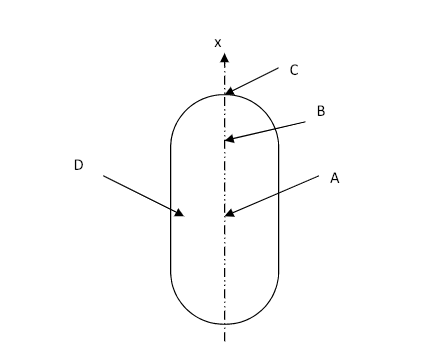
\includegraphics{vessel}


% Explain each rosette, angles, and possible similarities. 


\paragraph{Test Procedure}
Starting at 0 psig, a hand pump was used to increase the pressure by 50 psig. Once the pressure was set, a mean strain gage was shot selected, capturing an instantaneous state of strain. At 0 psig, theoretically, there should
be zero stress and strain in the vessel. However, the gages work by voltage outputs and using the measurement
at 0 psig, the following measurements were taken as the difference in the state. For example, the reading 
at 50 psig would be subtracted from the reading at 0 psig, giving each set of data a "normalized" value. This process
was repeated for each strain measurement up to 400 psig. After the ascending measurements were taken, the 
hand pump had its pressure released, and the strain values from 400 psig to 0 psig were taken, in 50 psig 
increments, to determine the descending sets of data. 


\paragraph {Data Reduction Procedure }
The overall flow of data starts at nominal strains, transformed to plane strains, converted  to
principal strains, and finally, through Hooke's law, converted to principal stresses. Once the measured 
principal stresses were obtained, they can be classified as either hoop or axial stresses within the 
context of the pressure vessel.

\begin{align}
\epsilon_1 = \epsilon_x\cos^{2}\theta_1 + \epsilon_y\sin^{2}\theta_1 + \gamma_{xy}\cos{\theta_1}\sin{\theta_1} \\
\epsilon_2 = \epsilon_x\cos^{2}\theta_2 + \epsilon_y\sin^{2}\theta_2 + \gamma_{xy}\cos{\theta_2}\sin{\theta_2} \\
\epsilon_3 = \epsilon_x\cos^{2}\theta_3 + \epsilon_y\sin^{2}\theta_3 + \gamma_{xy}\cos{\theta_3}\sin{\theta_3} \\
\end{align}

Once the strain values $\epsilon_x$, $\epsilon_x$, and $\gamma_{xy}$ are calculated, the principal strains
are produced by the equations :
$$ \epsilon_{p1}, \epsilon_{p2} = \frac{\epsilon_x + \epsilon_y}{2} \pm
 \frac{1}{2} \sqrt{ { \frac{\epsilon_x - \epsilon_y}{2}}^2 + {\gamma_{xy}}^2 } $$


Principal strains lead directly to the principal stresses, given the material properties of the vessel,
in the equation:
$$ \sigma_{p1} = \frac{E}{1-\nu^2} \big[ \epsilon_{p1} + \nu\epsilon_{p2} \big] $$,
$$ \sigma_{p2} = \frac{E}{1-\nu^2} \big[ \epsilon_{p2} + \nu\epsilon_{p1} \big] $$
	% Explain excel data reduction.
	
	
\paragraph {Data Validity Checking} 
During this experiment, two validity checks were used. First, strain measurements were taken. Based on the
strain configurations in Figure X, rosettes 4 and 11, 5 and 10 should have identical values. Also, the 
equation 25+10+11 should give a ratio of 1. 


% ========== Results ==========
\section{Results and Discussion}\label{conclusions}
		% Include validity checks between strain gages.


% ========== Discussion section  ==========
\section {Conclusions and Recommendations}



% ========== References ==========
\section {References}


% ========== Appendices ==========
\section {Appendices}

\end{document}
